\documentclass[11pt]{article}
\usepackage[margin=1in]{geometry}
\usepackage{graphicx}
\usepackage{booktabs}
\usepackage{lineno}
\usepackage[hidelinks]{hyperref}
\usepackage[numbers,sort&compress]{natbib}
\makeatletter
\setlength{\@fptop}{0pt}
\makeatother
\title{Extreme heat exposure around documented high-rise building fires worldwide}
\author{Author names and affiliations to be confirmed}
\date{}
\begin{document}
\maketitle
\linenumbers
\begin{abstract}
High-rise building fires concentrate risk vertically, but whether short-lived extreme heat coincides with their occurrence worldwide remains unresolved. We assembled 239 documented events from 52 countries and regions during 2000--2026 and linked event locations to local weather, population and built-form data. A time-stratified case-crossover design compared each event day with same-weekday control days at the same location and within the same month, reducing confounding by place, season and long-term reporting differences. The prespecified ERA5-Land heatwave indicator was not positively associated with a documented event day (conditional odds ratio 0.72, 95\% confidence interval 0.24--2.18; $P=0.563$; 21 informative strata), and estimates varied in direction across heat definitions and an independent NASA POWER product. The event catalogue also reveals strong geographic and recent-period reporting concentration, precluding interpretation of raw annual records as incidence. This evidence architecture separates acute heat exposure from urban fabric and documentation processes and shows that a plausible climate--fire mechanism cannot substitute for an identifiable, adequately powered event contrast.
\end{abstract}
Urban fire activity is produced jointly by ignition opportunities, combustible materials, building systems, occupant behaviour and emergency response. Climate adds a temporally varying stressor to this already coupled system. A recent global analysis reported that fire frequency in cities generally rises with warming and explicitly considered building fires, although temperature responses differ among fire categories and climate regimes\citep{Shi2025}. Historical documentary evidence from China likewise identified temperature variability as a leading climate indicator of urban fire activity, while showing that war, urbanisation and firefighting capacity can override or modify the relationship\citep{Yao2024}. These studies motivate a global building-specific test but also show why an event list alone cannot identify a climate effect.

High-rise fires are a consequential test case. Vertical evacuation, façade pathways, smoke movement, access constraints and concentrated occupancy can turn a local ignition into a system-scale emergency. Field experiments show that route visibility and elevator-lobby configuration alter evacuation choices in a high-rise hotel\citep{Mossberg2021}, while large-scale façade experiments demonstrate how suppression configuration changes upward flame migration and emitted heat flux\citep{Meraner2024}. Yet the available cross-national event evidence is fragmented across official reports, fire-service summaries, journalism and curated compilations. Analyses of global disaster data show that consequence missingness varies with year, national income and event type, while cross-border news attention varies with hazard type, fatalities and social ties\citep{Jones2022,Fetzer2026}. Although these studies are not fire catalogues, they motivate treating the physical events and their documentation process as distinct scientific objects. Otherwise, changes in search effort, language coverage and digital reporting become indistinguishable from changes in risk.

Here we build an evidence-bounded global analysis of 239 documented high-rise building fires during 2000--2026. We make three contributions. First, we formalise event provenance and analysis cohorts rather than treating heterogeneous records as exchangeable. Second, we link each event to daily ERA5-Land weather and compare the event day with same-place, same-month and same-weekday controls in a time-stratified case-crossover design. Third, we place acute heat exposure within approximately 1-km population and built-environment context using GPW and GHSL, while keeping these static layers conceptually separate from the acute exposure contrast. The primary estimand is the within-location association between extreme-heat exposure and a documented event day; severity and urban-form analyses are secondary and explicitly vulnerable to selective reporting.

\section*{Results}
\subsection*{A documented-event atlas with an explicit reporting boundary}
The updated database contained 239 records dated from 2 August 2000 to 23 August 2026. Valid coordinates were available for 233 records spanning 52 countries and regions. After excluding invalid coordinates and externally triggered disasters such as aircraft crashes or warfare, 228 events remained in the extended cohort. Requiring a traceable official, institutional or news source and excluding exact duplicate candidates yielded 191 events in the core cohort. The complete table is retained so that exclusion decisions remain auditable rather than silently changing the scientific population.

Documented events were geographically uneven, with 94 records in Asia, 63 in Europe and 46 in North America, compared with 14 in Oceania, 13 in Africa and 9 in South America. Records were also concentrated in 2025--2026. We interpret this as a mixture of event occurrence, database expansion and digital-source availability, not as evidence of a recent global incidence surge. Figure~1 therefore maps event locations over population exposure but labels the temporal inset as recording intensity.

\begin{figure}[ht]
\centering
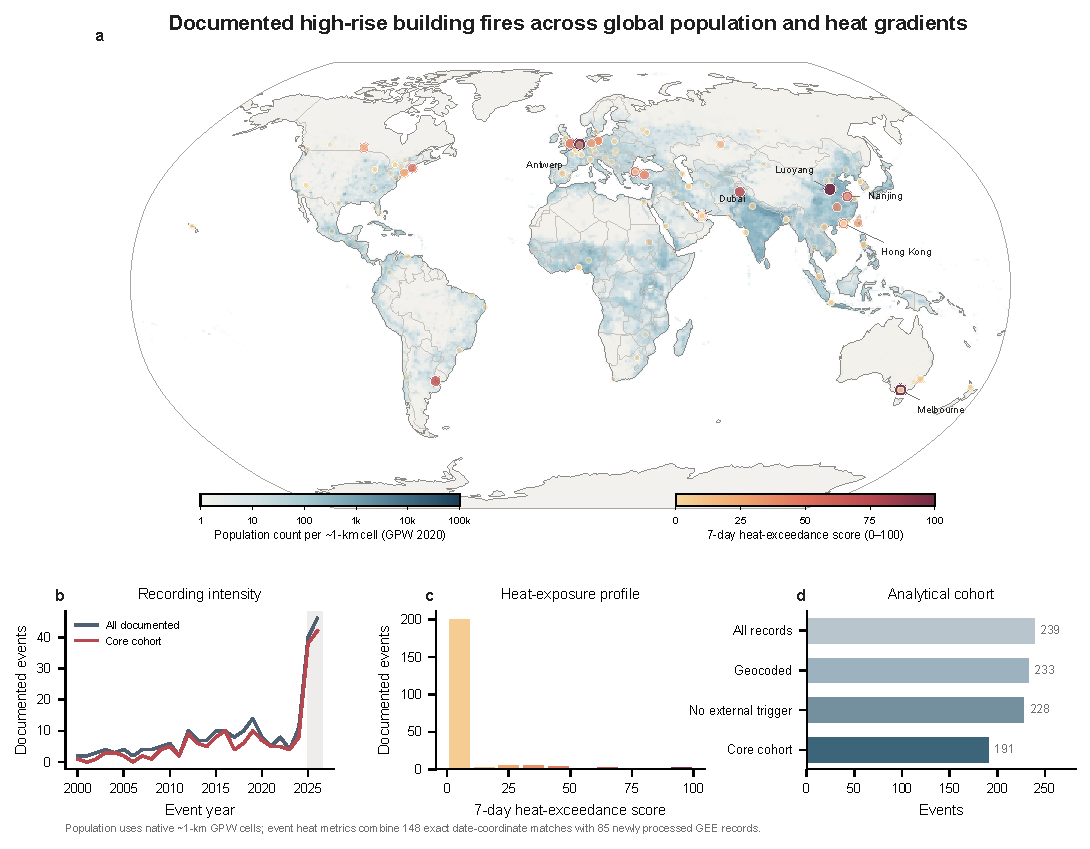
\includegraphics[width=\textwidth]{figures/Figure_1.pdf}
\caption{\textbf{Global distribution and evidence structure of documented high-rise building fires.} \textbf{a}, Event locations over the GPWv4.11 2020 population-count surface at its native approximately 1-km grid. Bubble colour and size show the descriptive 7-day heat-exceedance score; event-level heat metrics combine 148 exact date--coordinate legacy matches with 85 newly processed Earth Engine records. The five highest-scoring labelled cities and Hong Kong are annotated in black. \textbf{b}, Annual number of documented records for the full and core cohorts; the shaded recent period highlights potential database-expansion bias. \textbf{c}, Distribution of the descriptive heat-exceedance score. \textbf{d}, Prespecified cohort sizes. Map boundaries do not imply any position on legal status.}
\end{figure}

\subsection*{Acute heat exposure in matched event windows}
For each event in the extended cohort, the event day is compared with every other day of the same weekday in the same calendar month and year at the identical coordinate. This self-matched design removes all location characteristics that do not change within the month and controls calendar structure by design\citep{Levy2001}. Extreme heat is defined locally as at least three consecutive days whose daily maximum 2-m air temperature exceeds the larger of the 1991--2020 same-month 90th percentile and 30\,$^\circ$C. The ERA5-Land table contained 995 matched days in 228 strata. After adjustment for dewpoint, precipitation and wind, the primary heatwave indicator yielded an odds ratio of 0.72 (95\% confidence interval 0.24--2.18; $P=0.563$); only 21 strata contained within-stratum heatwave variation. Six prespecified definitions produced odds ratios from 0.33 to 1.21, with 12--46 informative strata, and every confidence interval included one (Fig.~\ref{fig:acute-heat}). These data therefore do not support a positive acute association, but the wide intervals also do not identify a precise null effect.

\begin{figure}[htbp]
\centering
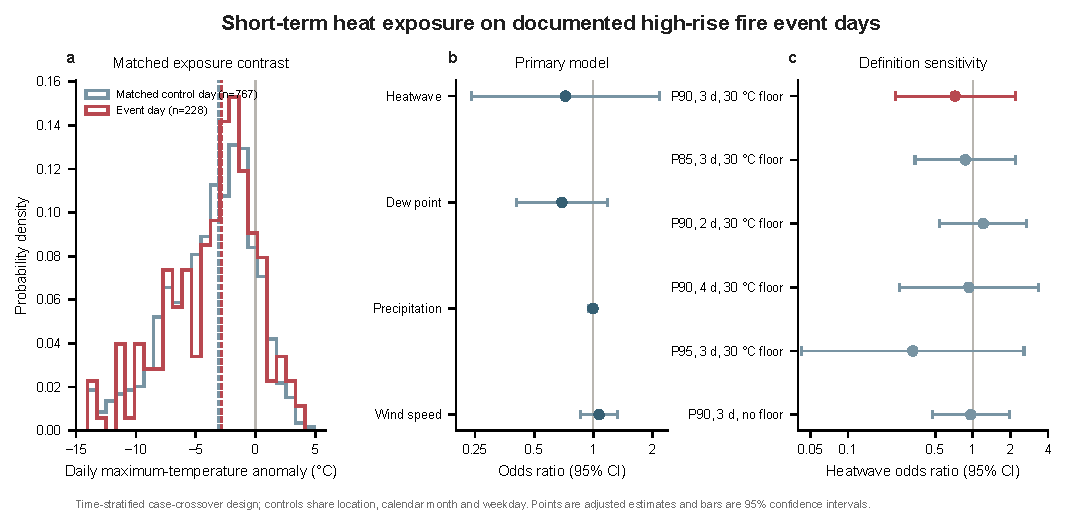
\includegraphics[width=\textwidth]{figures/Figure_2.pdf}
\caption{\textbf{Matched ERA5-Land evidence does not identify a positive acute heat association.} \textbf{a}, Distributions of daily maximum-temperature anomaly on 228 event days and 767 same-weekday control days; dashed lines mark medians. \textbf{b}, Adjusted odds ratios from the prespecified conditional logistic model for the binary heatwave indicator and time-varying weather covariates. Continuous covariates are scaled per interquartile-range increment. \textbf{c}, Heatwave odds ratios under six prespecified threshold, duration and absolute-floor definitions. Points show estimates and horizontal bars show 95\% Wald confidence intervals; all intervals include one. The primary definition contributes 21 informative strata, while alternatives contribute 12--46.}
\label{fig:acute-heat}
\end{figure}

An independent weather-product analysis used NASA POWER Release 10 for all 1,004 matched dates in 228 strata; 1,001 dates had complete heat, dewpoint, precipitation and wind fields for the adjusted models. On this coarser local-solar-time product, the primary heatwave definition yielded an odds ratio of 1.14 (95\% confidence interval 0.39--3.36; $P=0.807$), with 17 strata containing within-stratum exposure variation. Estimates across five alternative definitions ranged from 1.09 to 1.37, but every confidence interval included one and the number of informative strata ranged from 7 to 43 (Supplementary Fig.~S2). Thus, the product sensitivity was directionally positive but statistically imprecise; it neither confirms an association nor replaces the prespecified ERA5-Land analysis.

That directional pattern did not persist across every evidence restriction. The primary-definition estimate was 0.94 in the core cohort and ranged from 0.76 to 1.56 across leave-one-continent-out analyses; all intervals again included one (Supplementary Fig.~S5). The coarse-product result is therefore sensitive in direction as well as imprecise in magnitude.

This comparison answers a narrow question: whether documented events were more likely on locally extreme-hot days than on temporally matched days at the same place. It does not establish which ignition, material or behavioural mechanism operated in an individual fire. It also cannot correct events absent from the underlying catalogue. Negative-control and sensitivity analyses therefore test whether any estimated heat association survives exclusion of recent records, construction fires, arson and lower-grade sources.

\subsection*{Urban exposure and reported consequence}
Population count was sampled from the native GPW 2020 grid (30 arc-seconds; approximately 1 km), rather than multiplying a density surface by an arbitrary map pixel. GHSL built surface, building volume and mean height were summarized within an approximately 1-km neighbourhood. Recent fine-grid modelling in one Chinese urban district showed that population density and land-use composition can explain spatial concentration in recorded urban fires, but cannot by itself establish a global or short-term effect\citep{Wu2026}. Here these quantities describe people and built fabric potentially co-located with an event; they are not annual denominators and do not identify building occupancy at the time of fire. Among 66 core-cohort events with both deaths and injuries numerically reported and complete covariates, a secondary negative-binomial model gave a rate ratio of 1.04 per 10 points of the descriptive heat score (95\% confidence interval 0.90--1.21; $P=0.608$), adjusted for local population, built volume and event year. Missing deaths or injuries were never recoded as zero. The result is exploratory and does not support a heat--severity association in this selected complete-case sample.

Country-year GDP per capita, urban population share, electricity access and national population were added from the World Bank for contextual stratification. Historical values from the event year or at most three preceding years were permitted; 237 of 239 events were matched. These variables are not included in the self-matched occurrence model because they do not vary within an event stratum. Their role is to probe whether reported severity and database coverage differ systematically with development and infrastructure context.

\subsection*{The observation process is not random}
In a descriptive observation-process analysis with complete country-year context ($n=221$ extended-cohort events), 158 records contained a numeric injury count and 42 contained a numeric evacuation count. After adjustment for event year, continent and source grade, an interquartile-range increase in log GDP per capita was associated with higher odds that injuries were numerically reported (odds ratio 2.58, 95\% confidence interval 1.48--4.49; $P=0.00084$). Grade-C sources had lower injury-reporting odds than grade-A sources (0.30, 0.10--0.88; $P=0.028$). Evacuation reporting rose strongly with event year (odds ratio 4.46 per 10 years, 1.91--10.43; $P=0.00055$) and was also lower in grade-C than grade-A sources (0.12, 0.02--0.78; $P=0.026$). These estimates quantify documentation heterogeneity rather than fire risk, and show why complete-case severity results require explicit selection sensitivity.

\begin{figure}[htbp]
\centering
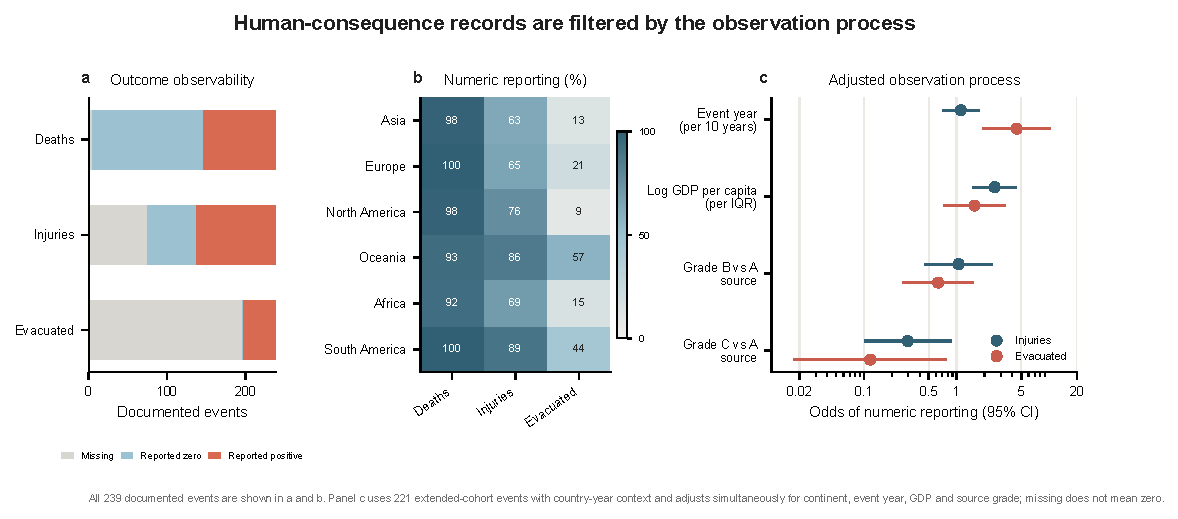
\includegraphics[width=\textwidth]{figures/Figure_3.pdf}
\caption{\textbf{Human-consequence records are filtered by the observation process.} \textbf{a}, Number of the 239 documented events with a missing, reported-zero or reported-positive value for deaths, injuries and evacuation. \textbf{b}, Percentage of records with a numeric value for each outcome by continent; percentages describe documentation completeness rather than event severity. \textbf{c}, Adjusted odds ratios for numeric injury and evacuation reporting in the 221-event extended-cohort analysis. Points show estimates and horizontal bars show 95\% Wald confidence intervals from separate binomial generalized linear models adjusted simultaneously for continent, event year, log GDP per capita and source grade. Missing outcome values were not recoded as zero. Panel-level source data are exported with the analysis.}
\label{fig:observation}
\end{figure}

\subsection*{Recorded consequences are concentrated and structurally heterogeneous}
Within the extended cohort, the 225 numeric death records contained 1,026 reported deaths and the 162 numeric injury records contained 2,031 reported injuries. These totals were highly concentrated across documented events: the Gini coefficient was 0.89 for deaths and 0.77 for injuries (Fig.~\ref{fig:consequence}). Positive-outcome proportions did not rise monotonically across quartiles of reported building size, underscoring that height or storey count alone does not order human consequence in this selected event set.

Exploratory adjusted models used records with a numeric outcome, country-year GDP and at least one reported building-size measure ($n=177$ for deaths and $n=127$ for injuries). Numeric injury records were weighted by the inverse of their estimated reporting probability; death records were unweighted because 98.7\% of extended-cohort records contained a numeric death value. The strongest contrasts were lower recorded injury-plus-one ratios for later event years (0.53 per 10 years, 95\% confidence interval 0.32--0.87; $P=0.013$) and façade fires (0.25, 0.11--0.57; $P=0.00097$), and a lower recorded death-plus-one ratio with higher log GDP per capita (0.60 per interquartile-range increment, 0.38--0.95; $P=0.028$). These conditional associations are neither incidence effects nor evidence that a fire type or economic setting is protective; they can also reflect event composition, outcome recording, evacuation, survival and residual selection.

National fire-service capacity data covered 141 extended-cohort events in 26 countries for firefighter metrics, with lower coverage for stations and engines. Across eight separate capacity--outcome sensitivity models, every 95\% confidence interval included one (Supplementary Fig.~S4). The non-common-year national data and sparse geographic support make this a coverage diagnostic, not evidence that response capacity has no effect.

\begin{figure}[htbp]
\centering
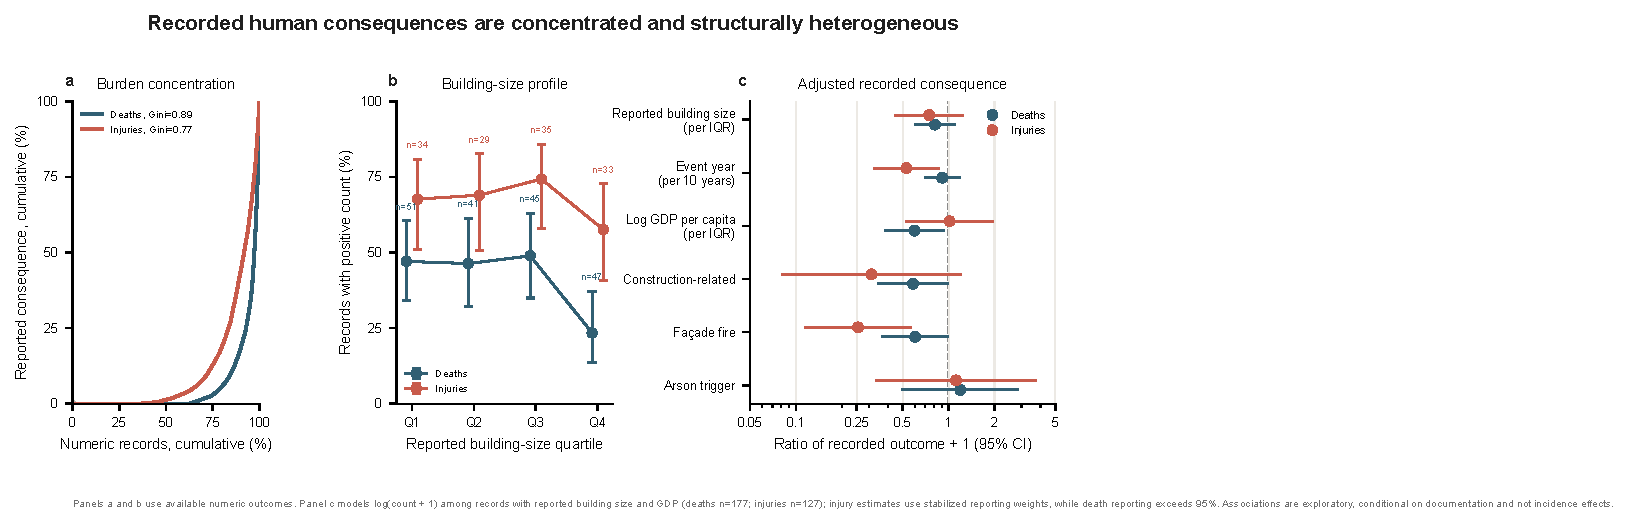
\includegraphics[width=\textwidth]{figures/Figure_4.pdf}
\caption{\textbf{Recorded human consequences are concentrated and structurally heterogeneous.} \textbf{a}, Concentration curves for numeric death ($n=225$) and injury ($n=162$) records in the extended cohort; the diagonal denotes equal distribution and labels give Gini coefficients. \textbf{b}, Percentage of numeric records with a positive death or injury count across quartiles of reported building size, constructed from the mean percentile rank of available height and storey count. Points show proportions, bars show 95\% Wilson intervals and labels give numeric-outcome denominators. \textbf{c}, Exploratory ratios of recorded outcome plus one from adjusted log-linear models. The death model used 177 records and equal weights; the injury model used 127 records and stabilized inverse-probability weights for numeric reporting. Both models adjusted simultaneously for all displayed terms, source grade and continent; points show estimates and bars show 95\% heteroskedasticity-consistent confidence intervals. Analyses are conditional on documentation, and no multiplicity-adjusted claim is made.}
\label{fig:consequence}
\end{figure}

\section*{Discussion}
This study reframes a heterogeneous global event compilation as an auditable exposure study. Its central innovation is not a more elaborate curve through event-only points, but a counterfactual comparison: weather on the observed event day versus plausible non-event days at the same location and season. That design aligns the estimand with the temporal scale at which heat can stress electrical demand, cooling equipment, human behaviour and material conditions while absorbing stable differences in climate, building stock, regulation and reporting culture.

The contrast between ERA5-Land and NASA POWER is itself a central result. The ERA5-Land primary estimate was below one, whereas NASA POWER estimates were above one across the prespecified definitions; both products yielded wide intervals because extreme-heat sequences varied within only a small fraction of matched strata. The approximately 50-km POWER grid and local-solar-time aggregation can also classify short heat sequences differently from ERA5-Land. Product choice therefore changes the point-estimate direction, and neither analysis provides decisive evidence of a positive association.
ERA5-Land evidence-window and leave-one-continent-out refits reinforce the information limit rather than recover a hidden positive effect. All 12 models converged and all intervals included one; exclusion of the five strata using a 20-km coastal fallback yielded an odds ratio of 0.77 (0.25--2.36). This pattern argues for prospective, harmonised event registration and denser exposure validation rather than selecting the heat definition or reanalysis that produces the preferred sign.

The approach also separates three quantities often collapsed in risk maps. Acute weather exposure varies by day; population and built volume represent the exposed urban substrate; documentation probability determines whether an event enters the database and which outcomes are recorded. The first can be tested within place, the second can contextualise consequence, and the third must be confronted through provenance and sensitivity rather than hidden. The observed GDP, source-grade and time gradients in injury or evacuation reporting confirm that consequence missingness is structured. This separation is essential because prior global and China-wide studies show both climatic and anthropogenic influences on urban fires\citep{Shi2025,Yao2024}.

The recorded consequence analysis adds a resource-planning signal without converting the event catalogue into an incidence denominator. A small fraction of documented events accounts for most reported deaths and injuries, so planning around an average event will understate tail demand. At the same time, lower adjusted recorded outcomes for façade fires, later injury records or higher-GDP death records must not be read as protective effects. These contrasts are conditioned on event discovery, numeric reporting and available building size, and may encode evacuation practice, survivorship, incident type and differential detail in sources. Their defensible role is to identify strata for prospective registry design and sensitivity analysis, not to rank jurisdictions or building systems.

This boundary also distinguishes our resource analysis from operational prediction. A recent one-city model used building, temporal and GIS features to predict fire escalation and simulate dispatch decisions\citep{Lee2025}; our CTIF analysis instead asks whether sparse national capacity context materially changes recorded-consequence associations. Its wide intervals and non-common reference years preclude operational or cross-national effectiveness claims.

Several limitations remain irreducible with the present data. The catalogue over-represents severe and searchable events, source availability differs by country and language, and recent years reflect active expansion. Static 2018/2020 population and built layers are temporally mismatched to early events. ERA5-Land represents neighbourhood-scale weather rather than indoor conditions or façade temperature. Fatalities, injuries and evacuations are inconsistently reported, and building age and height fields sometimes combine numeric and narrative information. The primary occurrence estimate is imprecise and product-sensitive, and the severity analysis is restricted to a selected 66-event complete-case sample. Neither result estimates the population incidence of high-rise fire.

The policy implication is methodological before it is operational. Short-term heat forecasts should not yet be used to reallocate high-rise fire resources on the strength of this catalogue alone. Agencies can instead register all eligible incidents prospectively, preserve zero as distinct from missing, link dispatch and building-system data, and predefine local heat contrasts; this would directly increase informative strata and test whether the global null-leaning estimate masks place-specific vulnerability. Existing work shows that strategic fire-protection investment involves explicit efficiency--equity trade-offs\citep{Behrendt2019}; population and vertical built volume can inform exposure context, but local operational evidence is required before heat-triggered allocation.

\section*{Methods}
\subsection*{Event database and provenance}
The source workbook contains one row per documented event and 21 author-curated fields covering location, date, sources, building characteristics, casualties, cause, spread and resilience gaps. The immutable input snapshot is identified by SHA-256 prefix \texttt{386eb5561012}; the complete digest is distributed in the machine-readable audit manifest. Dates and coordinates were parsed under explicit validity rules. Numeric casualties were extracted only when a number was reported; missing values were not converted to zero. Building height and storey count were parsed into separate fields only when metre or floor units were explicit, preventing areas and unlabelled numbers from being treated as height. Source domains were recorded, event identifiers were generated after stable chronological sorting, and all inclusion flags were preserved in the processed event table.

The all-event cohort retains every row. The extended cohort requires a valid date and coordinate and excludes fire directly triggered by aviation accidents, missiles, warfare or similar external disasters. The core cohort additionally requires a traceable official, institutional or news source and excludes exact date--coordinate--name duplicates. Construction, façade and arson indicators are retained for stratification rather than universally excluded.

\subsection*{External geospatial data}
Daily maximum 2-m air temperature, 2-m dewpoint, precipitation and 10-m wind components came from ERA5-Land Daily Aggregated in Google Earth Engine\citep{MunozSabater2021}. Weather was sampled from the ERA5-Land pixel at the event coordinate. If the land mask returned no value for a coastal coordinate, all dates in that stratum used a documented 20-km buffer mean; this affected five of 228 strata and was tested by complete exclusion. GPWv4.11 supplied 2020 population count and density at 30 arc-seconds\citep{GPW2020}. GHSL P2023A supplied 2020 built surface and building volume, 2018 mean building height at 100 m, and 2020 degree of urbanisation at 1 km\citep{GHSL2023}. Built variables were summarized in an equal-area neighbourhood of approximately 1 km$^2$ around each event.

For independent weather-product sensitivity, the NASA POWER Daily API supplied maximum 2-m air temperature, 2-m dewpoint, corrected precipitation and 10-m wind speed in local solar time\citep{Gelaro2017,NASAPOWER2026}. POWER Release 10 derives meteorological fields from MERRA-2 and appends low-latency GEOS-IT data near real time. We queried one time series per unique coordinate from 1 January 1991 through the later of 31 December 2020 and the latest matched date, using API version v2.9.7 returned at access on 31 August 2026. The native meteorological grid is 0.5\,$^\circ$ latitude by 0.625\,$^\circ$ longitude. The same fixed baseline, threshold, duration and matched-day algorithms were then applied independently of the Earth Engine extraction. Dates within two months of access were flagged as provisional; this affected 68 matched-day rows and no value was silently discarded.

For cross-sectional response-capacity sensitivity, CTIF World Fire Statistics Report No.~30 Table~1.13 supplied national fire-station, engine and firefighter counts for 65 countries\citep{CTIF2025}. Values are each country's most recent report during 2010--2023 rather than a common-year series. Counts were divided by the table's national population to derive per-100,000-person metrics; they were not treated as time-varying event exposures.

World Development Indicators were downloaded through the World Bank API\citep{WorldBank2026}. Country names were normalized to ISO3 codes. For each event, the event-year value or the most recent prior value within three years was used. No forward-year imputation was allowed.

\subsection*{Heatwave definition}
The primary relative threshold is the location-specific 90th percentile of daily maximum temperature during 1991--2020, with seasonality represented in the current implementation by the event calendar month. A 30\,$^\circ$C absolute floor prevents mild relative anomalies in cool climates from being labelled high thermal load. A heatwave day requires the current and two preceding days all to exceed the larger threshold. Three-day, percentile-based definitions are widely used in global heatwave research\citep{PerkinsKirkpatrick2020}. Implemented sensitivity analyses use P85/P90/P95, two to four consecutive days and removal of the absolute floor; calendar-day windows and excess heat factor are reserved for future extensions and are not reported as completed analyses.

The map-only score summarizes the seven-day event window as ten times cumulative degree-days above the compound threshold, truncated to 0--100. It is a descriptive visual index, not a probability, percentile, causal effect or validated fire-danger scale. The event-day temperature percentile is stored separately.

\subsection*{Time-stratified case-crossover analysis}
Each event defines one stratum. Control days are all other days with the same weekday in the same month and year, at the event coordinate. Conditional logistic regression estimates the odds of an event day as a function of the binary heatwave indicator while conditioning on stratum. The binary exposure remains on its original 0/1 scale, so its coefficient compares exposed with unexposed days; dewpoint, precipitation and wind are scaled per interquartile-range increment. Because location is fixed within stratum, population, built form, country, climate zone and stable reporting propensity cancel from the occurrence contrast. Separate robustness models replace the primary exposure with prespecified heatwave thresholds and durations and exclude event categories listed in Supplementary Table~S1.

For both ERA5-Land and the independent NASA POWER product, the primary definition was additionally refitted in the core cohort, after excluding 2025--2026, construction, façade or arson records, and after leaving out each continent in turn. Each restriction preserved complete event strata, used the same time-varying covariates and reported the number of strata with within-stratum heatwave variation. Failed or non-identifiable fits were retained with status codes rather than omitted. An additional ERA5-Land sensitivity excluded every stratum requiring the coastal spatial-mean fallback.

\subsection*{Severity and heterogeneity analyses}
Reported deaths and injuries are summed only when both underlying fields contain a numeric value; an explicitly reported zero remains distinct from missing information. The GEE-linked exploratory count model uses a negative-binomial mean structure with heteroskedasticity-consistent uncertainty. To avoid unstable adjustment for sparse categories in 66 complete cases, its prespecified parsimonious adjustment set contains the descriptive heat score per 10 points, log population, log built volume and event year per decade. The score is a map-oriented exposure summary, so this model is secondary and is not interpreted as the occurrence estimand.

An available-data heterogeneity analysis was specified separately. Reported building size is the mean within-dataset percentile rank of explicit metric height and explicit storey count when both are available, or the available rank when only one is reported; it is a relative evidence variable, not an imputed physical height. Deaths and injuries are modelled separately after transformation as $\log(\mathrm{count}+1)$, with reported building size and log GDP scaled per interquartile range, event year scaled per 10 years, and construction, façade, arson, source-grade and continent terms entered simultaneously. Injury models use stabilized inverse-probability weights from the numeric-reporting model\citep{Cole2008}, predicted probabilities truncated to 0.05--0.995 and weights winsorized at the first and 99th percentiles. Deaths use equal weights because numeric reporting exceeds 95\%. Weighted least squares uses HC3 standard errors; exponentiated coefficients are ratios of the geometric mean of recorded outcome plus one. This procedure assumes that measured reporting covariates are sufficient for the weighting model, does not address missing building size and remains exploratory.

The response-capacity sensitivity adds one log-transformed, interquartile-range-scaled CTIF metric at a time to the corresponding recorded-consequence model. Four separate metrics---career firefighters, all firefighters, fire stations and fire engines per 100,000 people---avoid an unsupported composite index. Each model reports its event and country denominator; no temporal or causal interpretation is assigned to these static national values.

\subsection*{Reporting and reproducibility}
Reporting completeness is modelled separately from physical outcomes. For injury and evacuation fields, a binary indicator denotes whether a numeric value was available, not whether the outcome occurred. Exploratory binomial generalized linear models include event year, log GDP per capita, source grade and continent; year and log GDP are scaled by their interquartile ranges, and heteroskedasticity-consistent standard errors are used. These models diagnose selection into analyzable consequence records and are not used to impute missing values.

All transformations are implemented in four STEP-labelled Jupyter notebooks and four Python modules. Code cells contain compact Chinese end-of-line comments to match the project convention. Every figure exports vector PDF/SVG, 600-dpi TIFF and panel-level CSV source data. Tests verify source hashes, cohort counts, required fields, notebook syntax and figure dimensions. Statistical tests are two-sided; effect estimates are reported with 95\% confidence intervals and exact analysis denominators. No adjustment is made for multiple testing in the prespecified primary model; secondary analyses are labelled exploratory.

\subsection*{Data availability}
The processed event table, cohort flags, panel-level source data and data-source registry will be deposited in a DOI-minting research repository before submission. Redistribution of source text and URLs will follow the terms of each source; where redistribution is restricted, row-level provenance and processing code will be shared so users can reconstruct eligible records. ERA5-Land, GPW, GHSL and World Development Indicators remain available from their respective providers under their stated licences. The service-account key is a credential and will never be archived.

The derived NASA POWER matched-day sensitivity table and a request manifest containing coordinates, intervals, API version, source stream, local-solar-time convention and access timestamps will be included after provider-terms review. Raw point-response caches are operational intermediates and are not part of the planned deposit. Near-real-time rows remain marked as provisional.

The CTIF-derived national-capacity table retains the source page, report URL and source-file checksum. Its redistribution will follow CTIF terms; otherwise, extraction code and row-level derivation metadata will be released without redistributing protected report content.

\subsection*{Code availability}
The Python notebooks, modules, environment specification, configuration and LaTeX sources are maintained at \url{https://github.com/fengjiawei126/global-high-rise-fire-map}; an immutable archival DOI will be added at publication. Earth Engine access requires the user's own authorised Google Cloud project and credentials. No credential file is included in the repository.

\section*{Acknowledgements}
To be completed by the authors. ERA5-Land data were generated using Copernicus Climate Change Service information. The European Commission and ECMWF are not responsible for any conclusions drawn from these data.

\section*{Author contributions}
To be completed using the CRediT taxonomy after the author list is confirmed.

\section*{Competing interests}
The authors declare no competing interests, subject to author confirmation.

\section*{Use of generative AI}
Generative AI was used for code scaffolding, language drafting and consistency checks under human supervision. All source selection, event coding, statistical decisions, numerical results and final claims require author verification. The tool is not an author.

\bibliographystyle{unsrtnat}
\bibliography{references}
\end{document}
